\section{\system Runtime}
\label{sec:system}

The runtime contains a contract registry, scheduler, monitor, artifact store, fault localizer, recovery controller, event log, and replay utilities. Before a node runs, the monitor checks dependency and precondition contracts. After execution, it checks schema and budget contracts and emits violations. The fault localizer maps violations into operational classes such as artifact, coordination, resource, tool-environment, runtime, and verifier faults. The recovery controller selects bounded actions such as quick repair, retry, reroute, rollback, invalidation, degradation, human escalation, or dead-letter.

Every event is traceable by task identifier and run identifier. Events include graph creation, contract checks, node scheduling, artifact production, violations, fault diagnoses, recovery decisions, checkpoints, rollbacks, dead letters, and task finalization.

\begin{figure}[t]
    \centering
    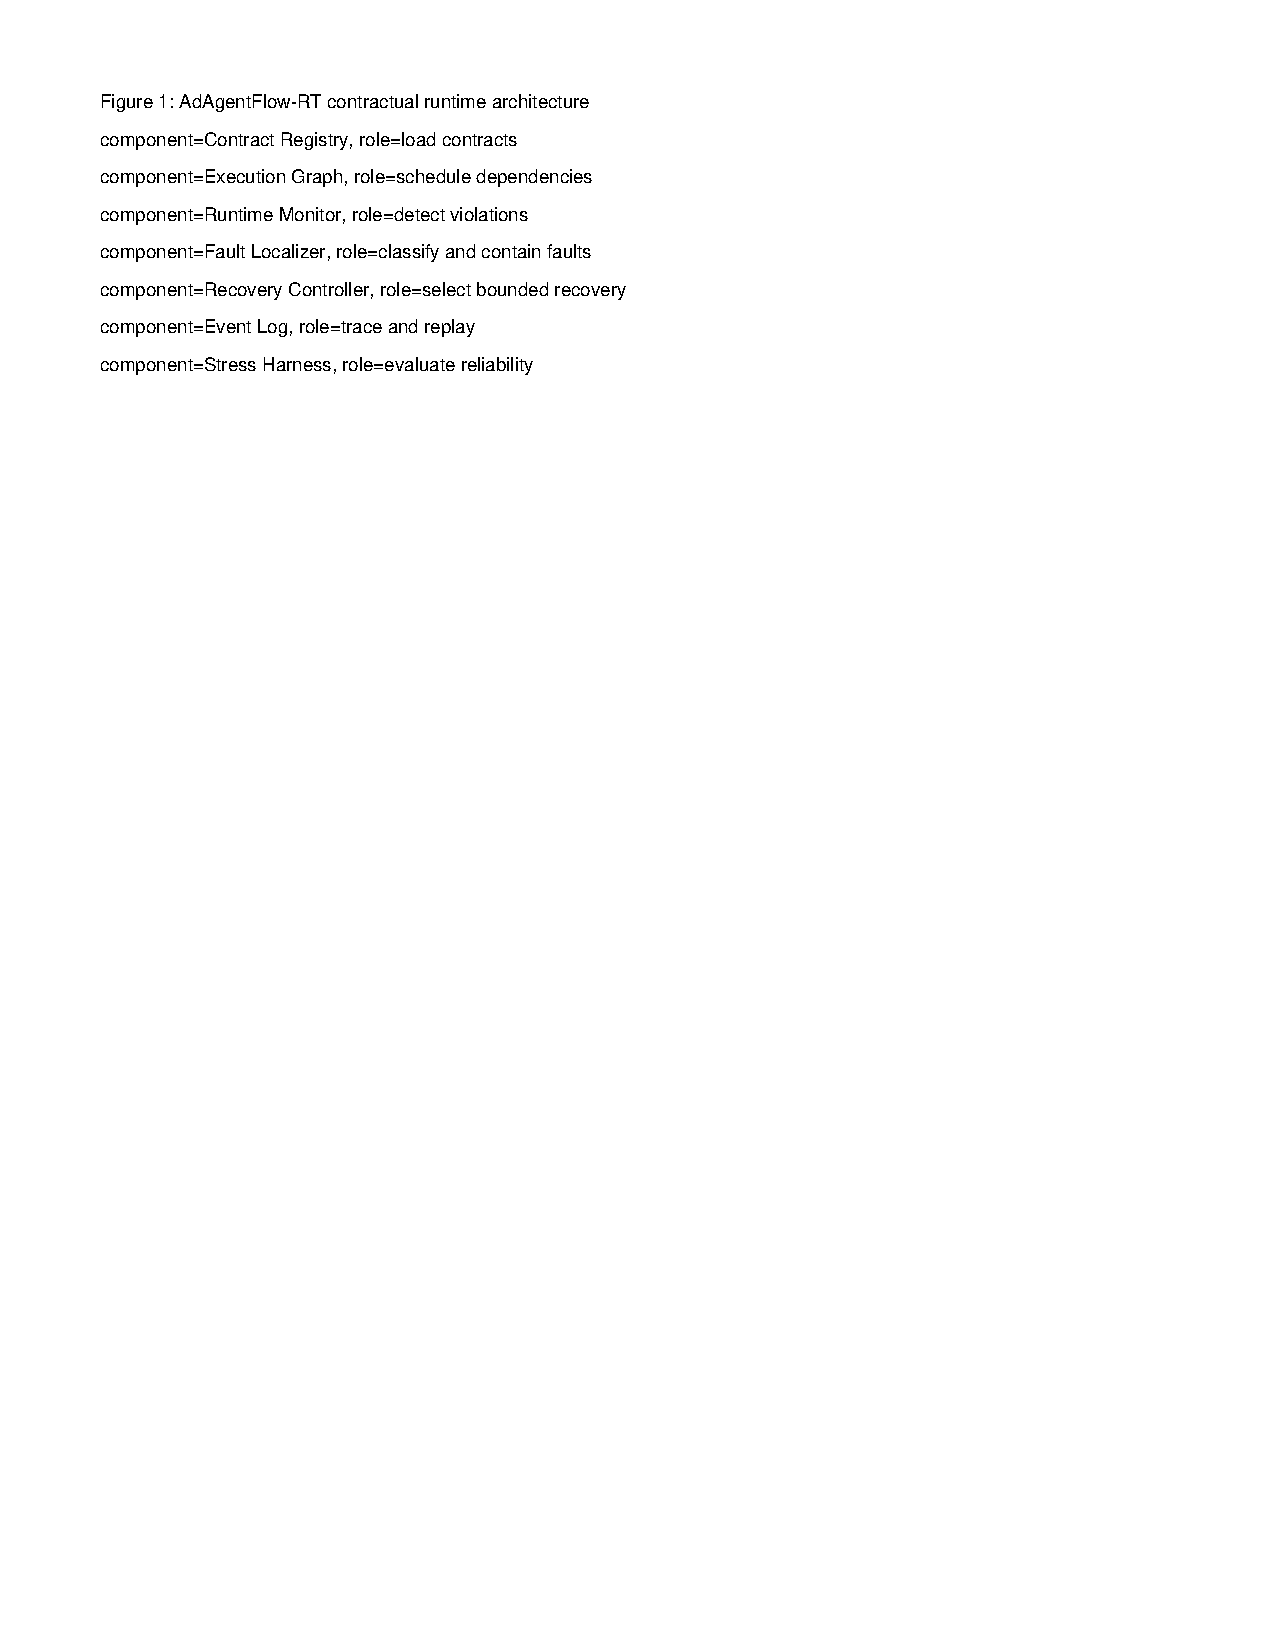
\includegraphics[width=\linewidth]{figs/system_architecture.pdf}
    \Description{A component diagram listing the contract registry, execution graph, runtime monitor, fault localizer, recovery controller, event log, and stress harness.}
    \caption{\system contractual runtime components.}
    \label{fig:system}
\end{figure}

\subsection{Runtime Kernel}

Figure~\ref{fig:system} shows the runtime components. The contract registry stores executable contract specifications. The graph planner constructs a dependency graph. The scheduler selects runnable nodes whose dependencies are satisfied. The monitor checks contracts before and after node execution. The artifact store records produced artifacts and validation status. The fault localizer maps violations into operational fault classes. The recovery controller selects bounded actions from policy and remaining budget. The event log records each runtime transition for replay and metric extraction.

\subsection{Event-Sourced Trace}

The event log records `graph.created', `contract.loaded', `node.started', `contract.checked', `fault.injected', `contract.violated', `fault.localized', `recovery.started', `recovery.selected', `recovery.succeeded', `artifact.produced', `dead\_letter.created', and `task.finalized'. Each event carries `task\_id', `run\_id', optional `node\_id', status, payload, and timestamp. The smoke harness also records relative millisecond offsets so trace metrics can estimate mean time to detect and recover.

\subsection{Runtime Strategies}

The harness implements four comparable strategies:

\begin{itemize}
    \item \textbf{Vanilla}: directly executes the benchmark-style task without runtime contracts or recovery.
    \item \textbf{Retry-only}: retries after failure until a bounded retry count is exhausted.
    \item \textbf{Schema-only}: validates schema and applies repair/retry, but does not localize graph-level faults.
    \item \textbf{\system}: applies contract monitoring, fault localization, bounded recovery, artifact invalidation hooks, dead-letter handling, and event trace.
\end{itemize}
